\documentclass[11pt]{article}

\usepackage{graphicx}
\usepackage{amssymb}
\usepackage{amsfonts}
\usepackage{amsmath}

\setlength{\parindent}{0pt}

\begin{document}

\section*{Aerodynamic simulation in SolidWorks Flow dink}

Solidworks flow simulation for a simplified version of the tandem trike (simple wheels, no chairs).
Increased ``global initial mesh refinement'' until results converge.

It is clear that predicted force $F$, and power $P$ calculated by $P = F v$ is low by a factor $\approx 3$. 

\begin{figure}[h!]
\centering
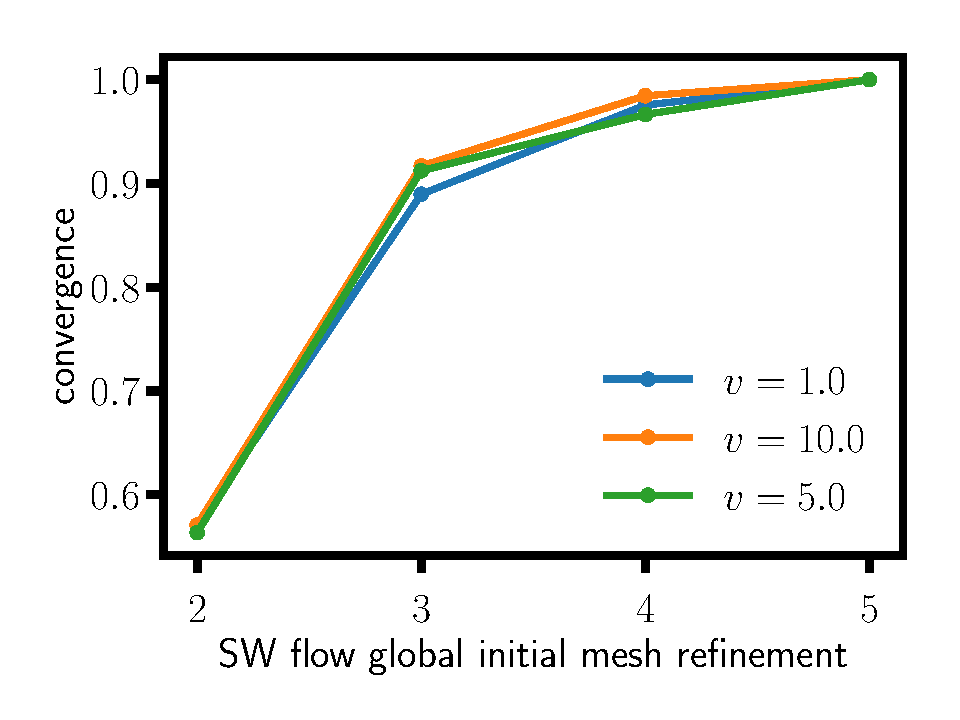
\includegraphics[width=0.55\textwidth]{convergence.pdf}
\end{figure}

\begin{figure}[h!]
\centering
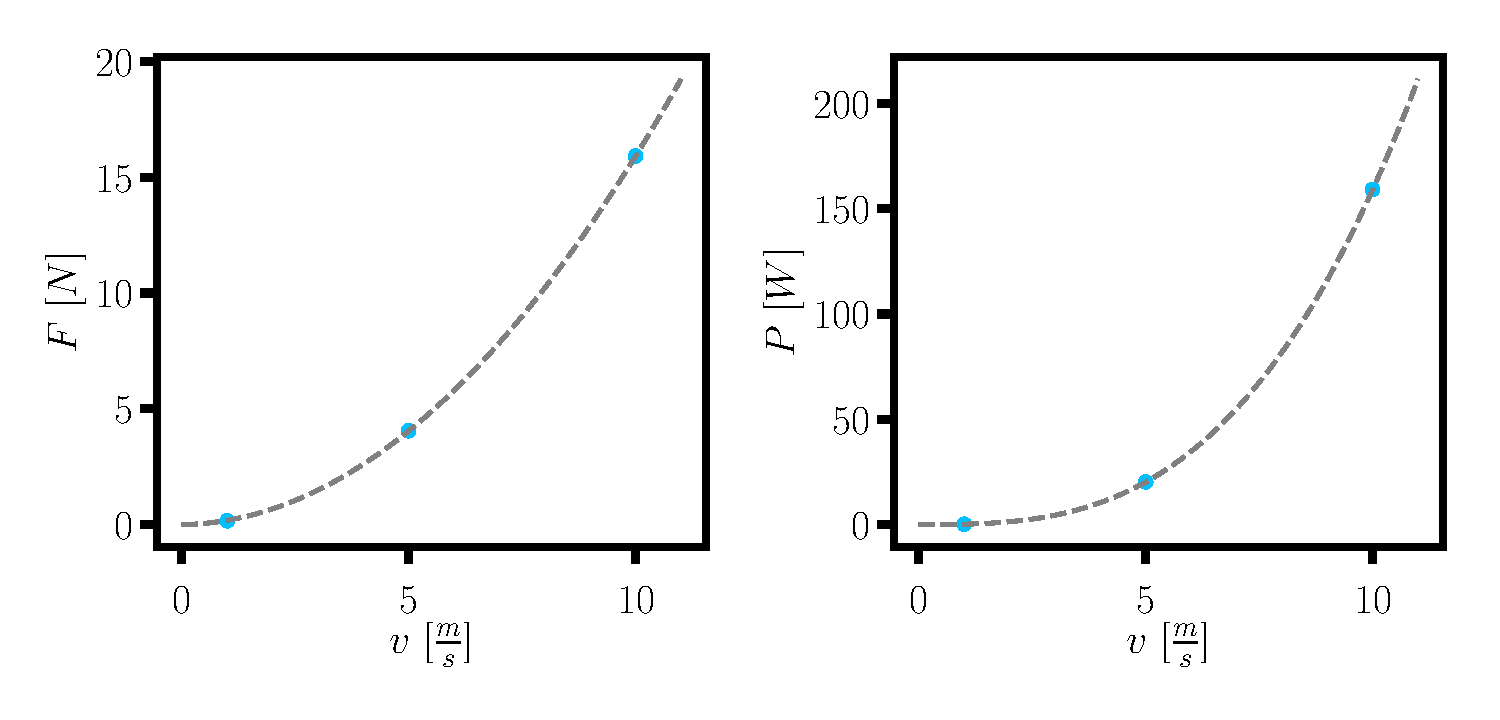
\includegraphics[width=\textwidth]{ForcePower.pdf}
\end{figure}

\section*{Sideview velocity contour plots}

\begin{figure}
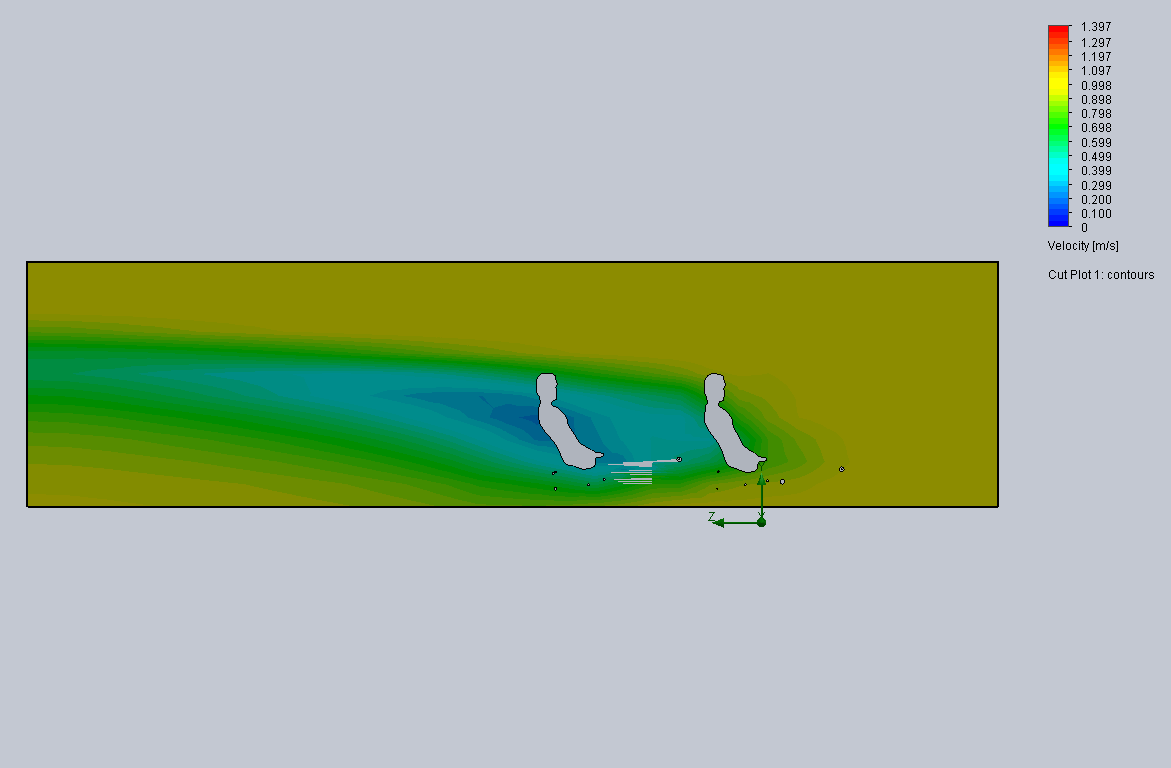
\includegraphics[width=\textwidth]{gm_2_rf_7_v01.png}
\caption{$v = 1 m/s$, global initial mesh = 2}
\end{figure}

\begin{figure}
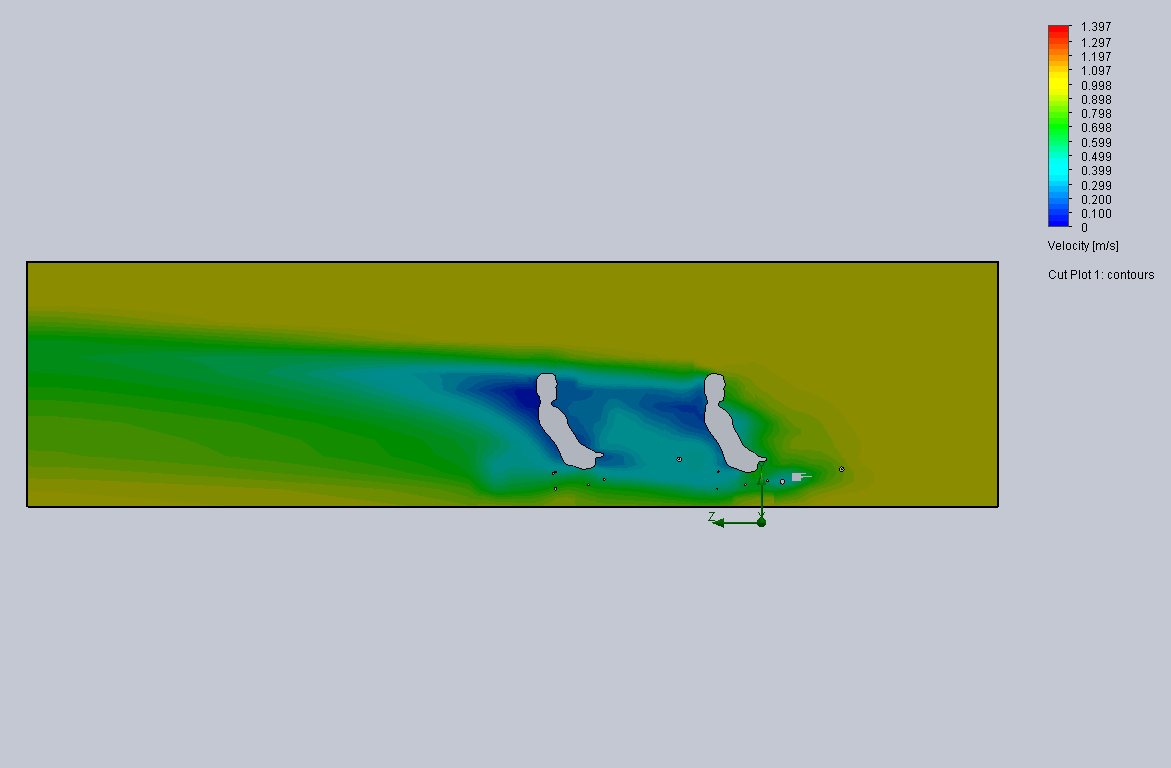
\includegraphics[width=\textwidth]{gm_3_rf_7_v01.png}
\caption{$v = 1 m/s$, global initial mesh = 3}
\end{figure}

\begin{figure}
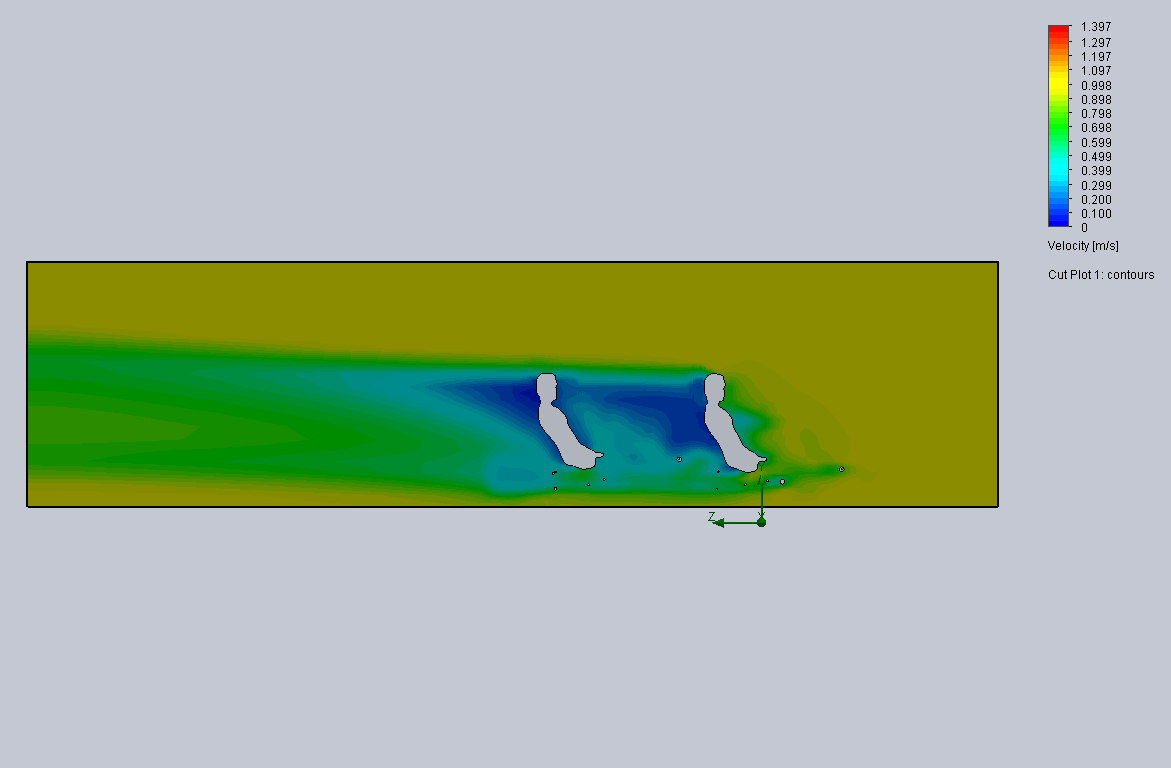
\includegraphics[width=\textwidth]{gm_4_rf_7_v01.png}
\caption{$v = 1 m/s$, global initial mesh = 4}
\end{figure}

\begin{figure}
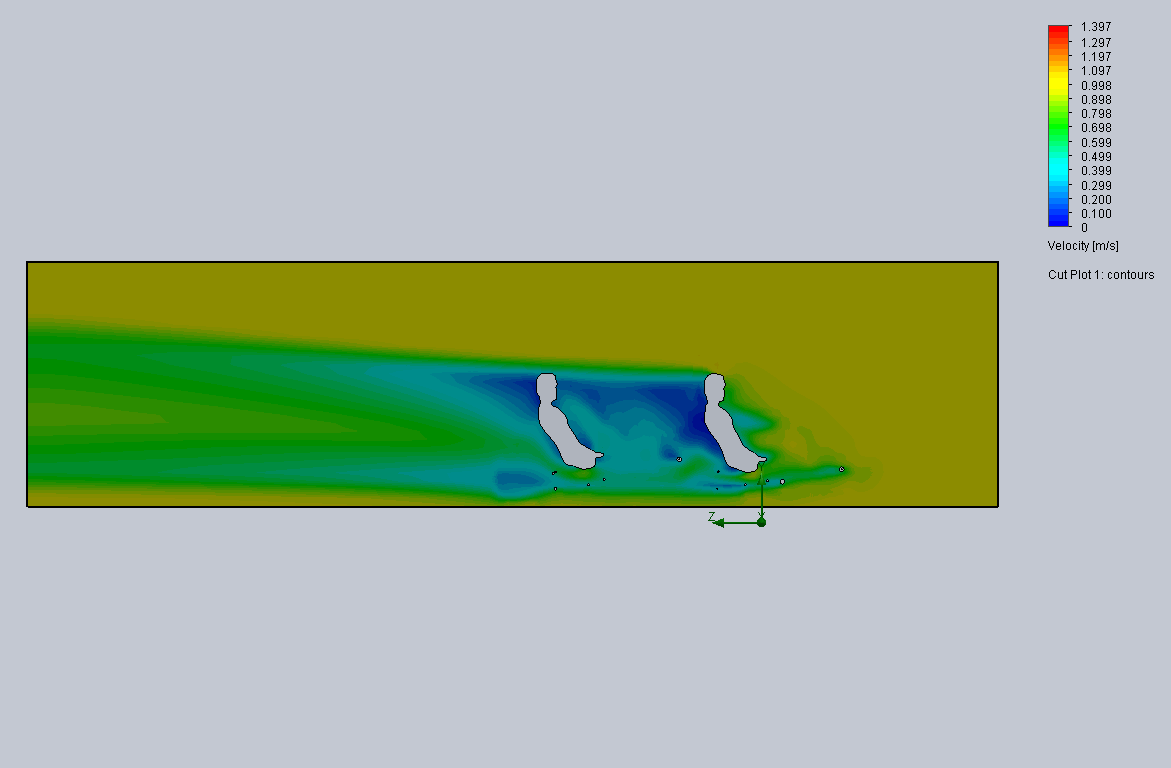
\includegraphics[width=\textwidth]{gm_5_rf_7_v01.png}
\caption{$v = 1 m/s$, global initial mesh = 5}
\end{figure}


\begin{figure}
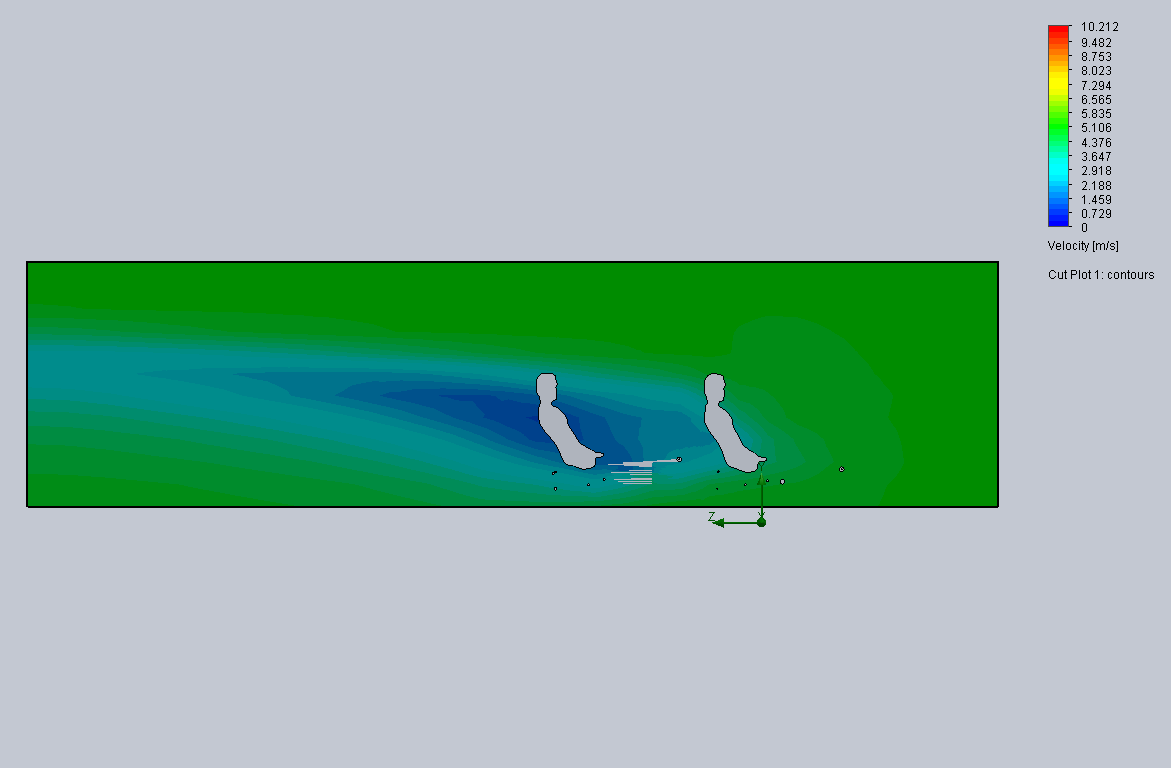
\includegraphics[width=\textwidth]{gm_2_rf_7_v05.png}
\caption{$v = 1 m/s$, global initial mesh = 2}
\end{figure}

\begin{figure}
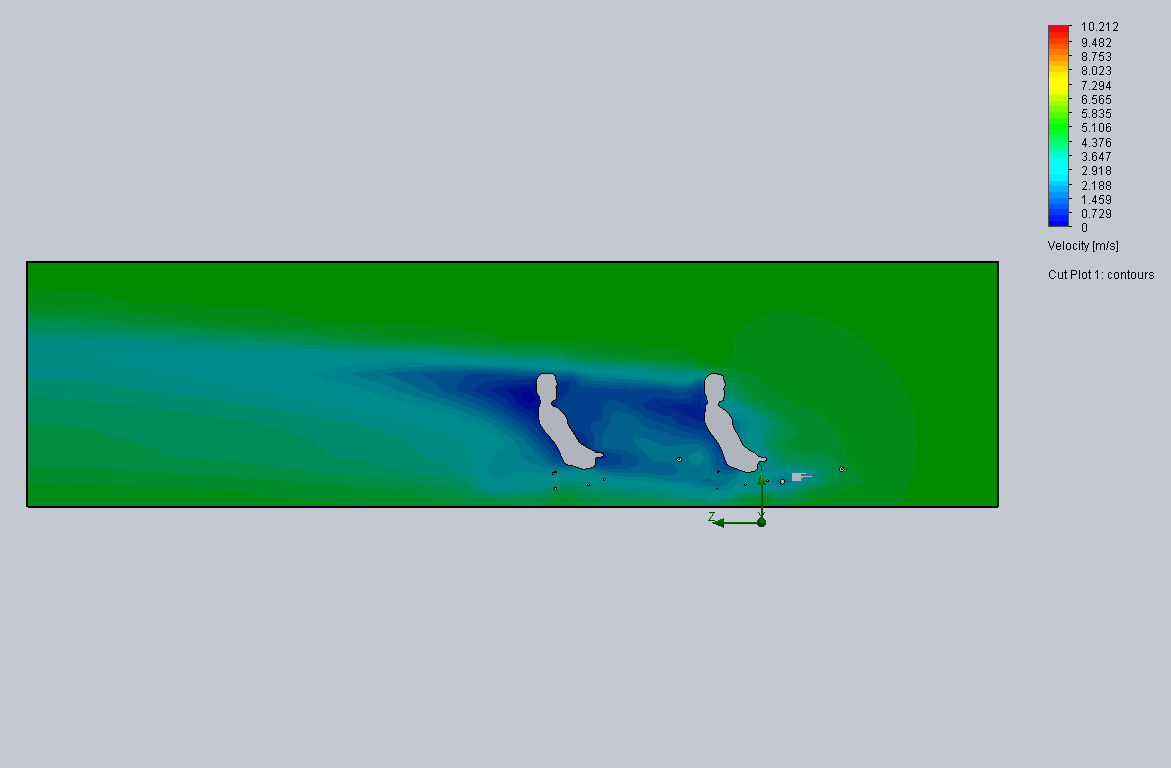
\includegraphics[width=\textwidth]{gm_3_rf_7_v05.png}
\caption{$v = 1 m/s$, global initial mesh = 3}
\end{figure}

\begin{figure}
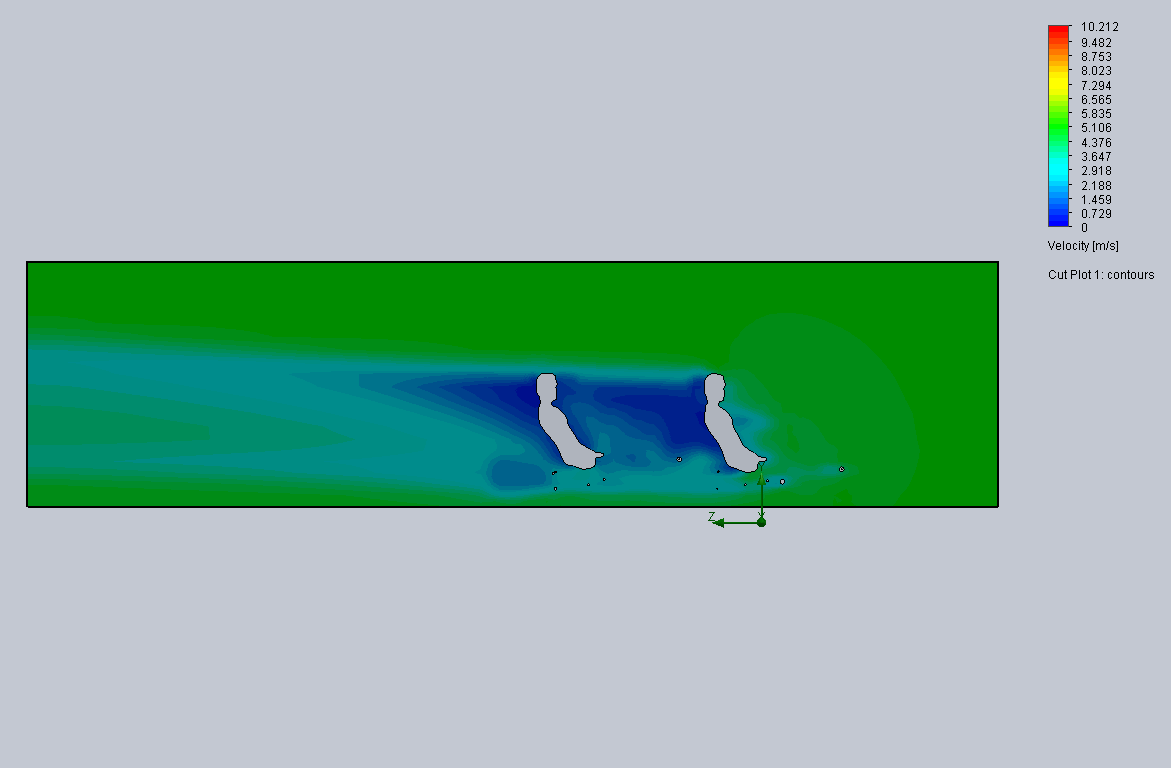
\includegraphics[width=\textwidth]{gm_4_rf_7_v05.png}
\caption{$v = 1 m/s$, global initial mesh = 4}
\end{figure}

\begin{figure}
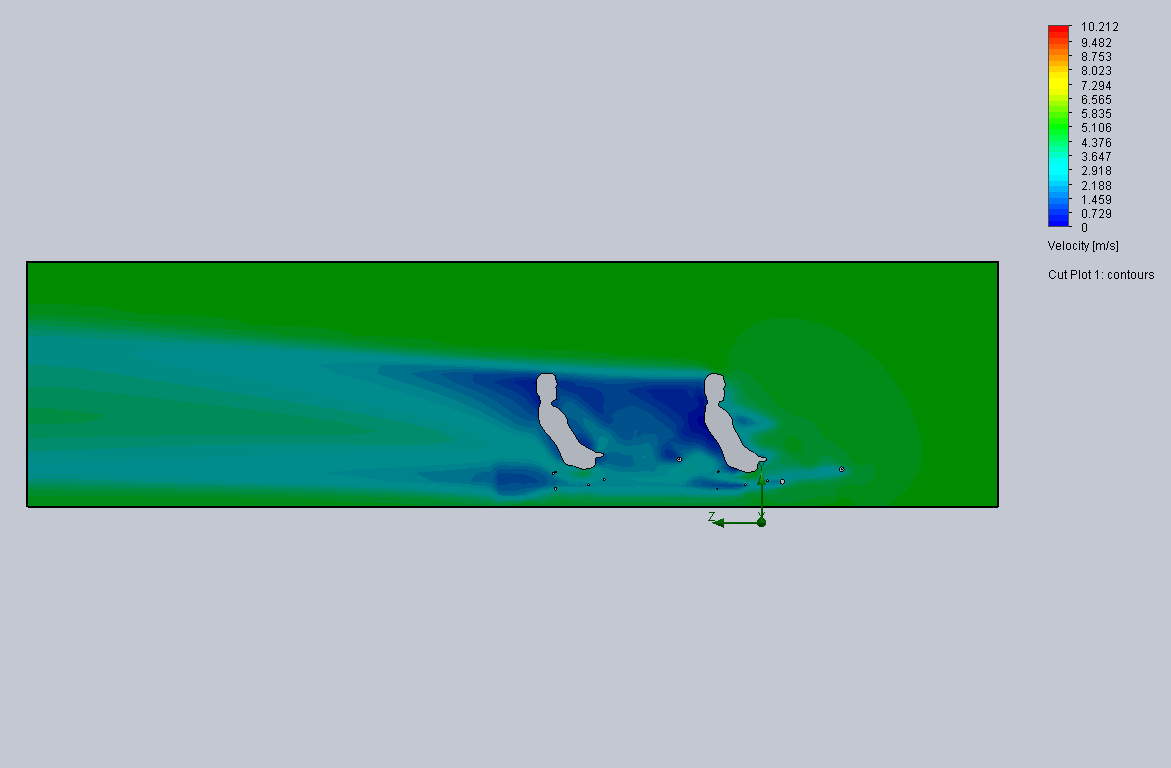
\includegraphics[width=\textwidth]{gm_5_rf_7_v05.png}
\caption{$v = 1 m/s$, global initial mesh = 5}
\end{figure}

\begin{figure}
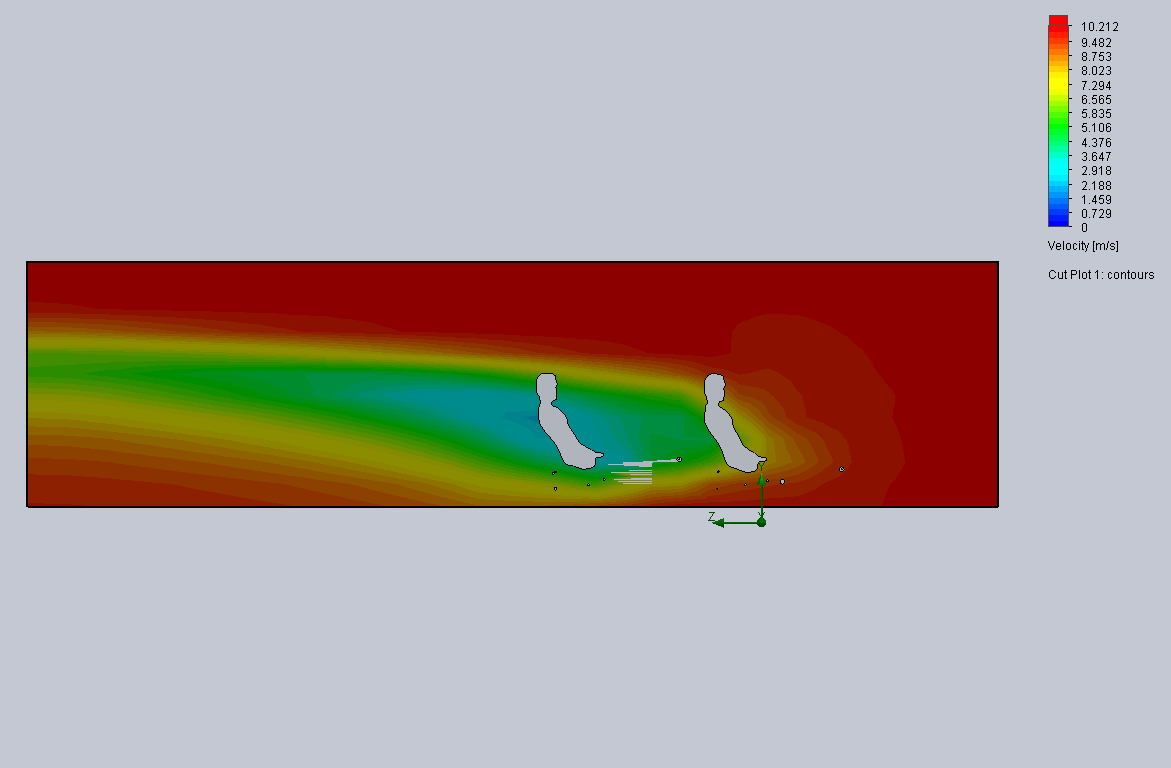
\includegraphics[width=\textwidth]{gm_2_rf_7_v10.png}
\caption{$v = 1 m/s$, global initial mesh = 2}
\end{figure}

\begin{figure}
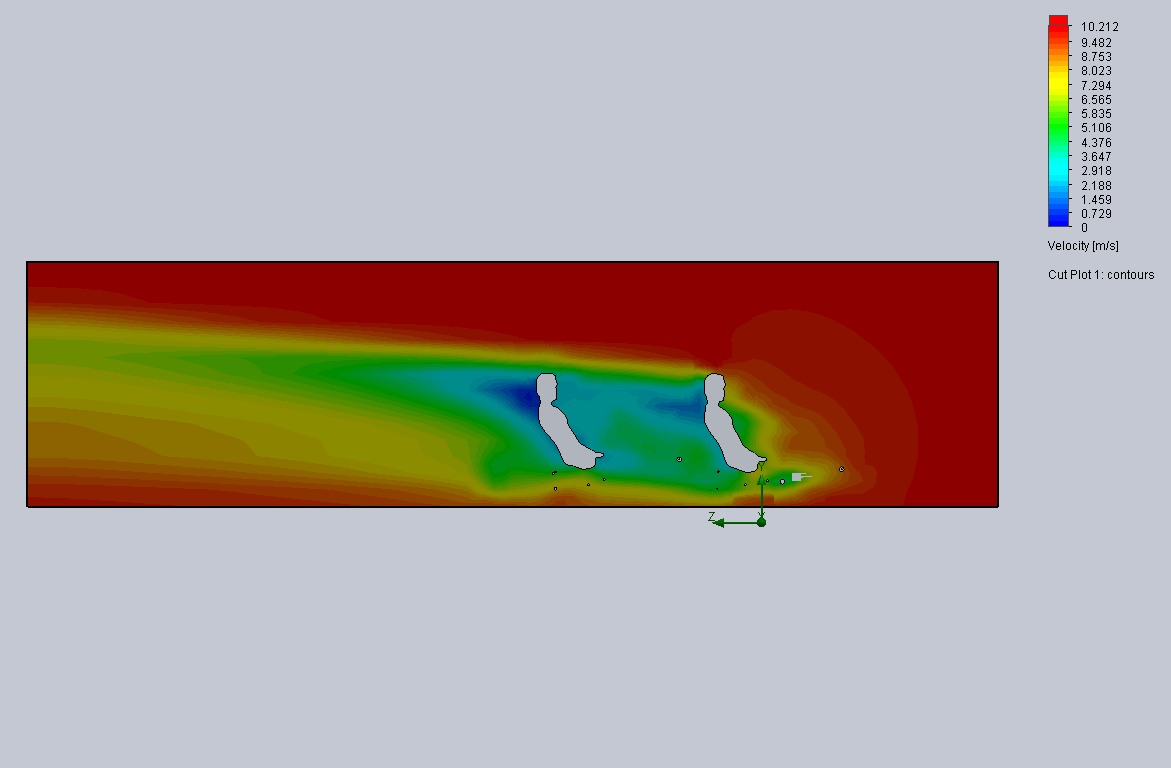
\includegraphics[width=\textwidth]{gm_3_rf_7_v10.png}
\caption{$v = 1 m/s$, global initial mesh = 3}
\end{figure}

\begin{figure}
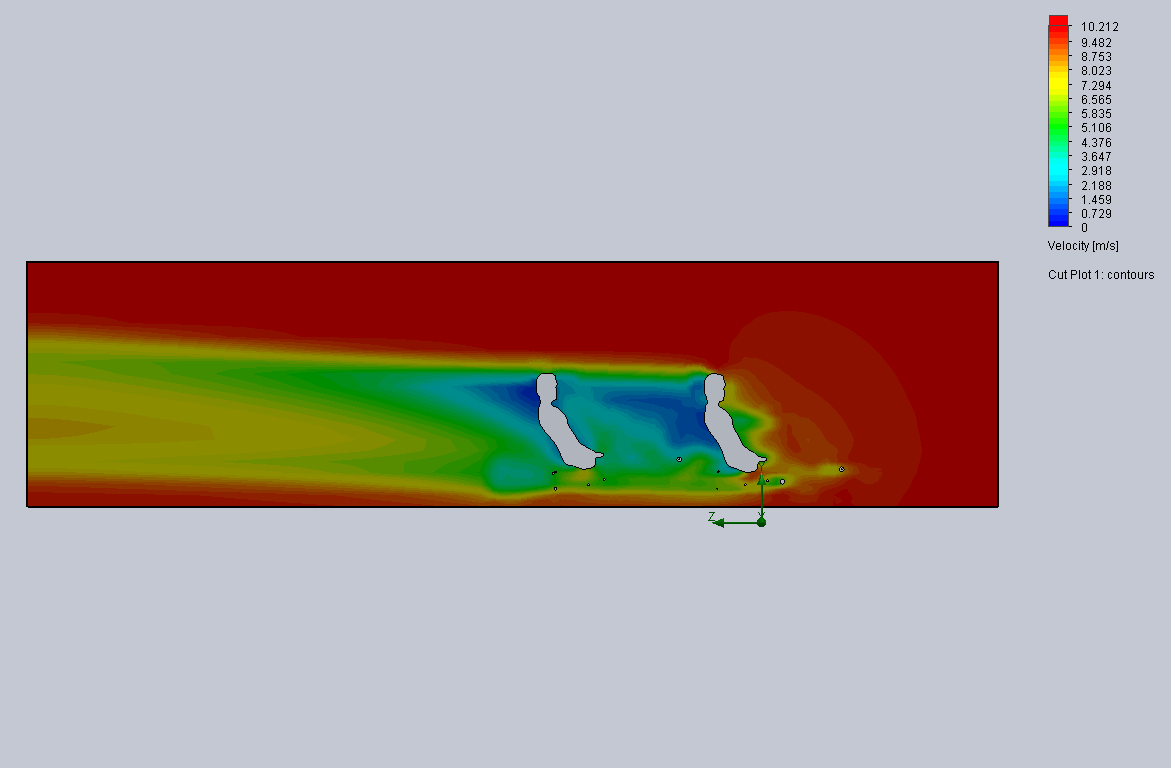
\includegraphics[width=\textwidth]{gm_4_rf_7_v10.png}
\caption{$v = 1 m/s$, global initial mesh = 4}
\end{figure}

\begin{figure}
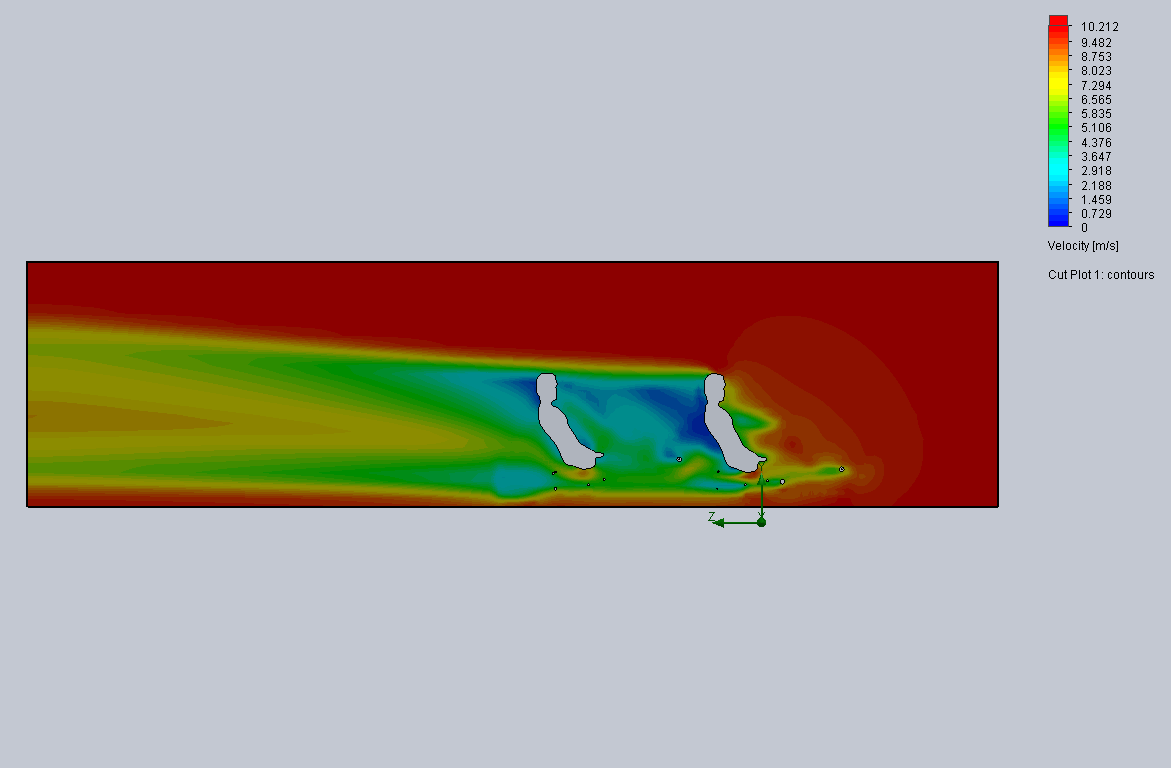
\includegraphics[width=\textwidth]{gm_5_rf_7_v10.png}
\caption{$v = 1 m/s$, global initial mesh = 5}
\end{figure}


\end{document}